\section{Experiments}

We evaluated SAMNet on the COG dataset and compared our results to the baseline model described in ~\cite{yang2018dataset}. To test the generalization ability of both models, we used the canonical (easy) and hard settings that alter the number of distractors and sequence length.  Since there was no baseline for these tests (train on canonical, test on hard), we ran our own experiments using the COG model provided by the authors.  SAMNet achieves the highest overall scores for all categories of experiments (\cref{tab:results}), especially for the tests run on the hard dataset.  Among the 22 classification tasks, we highlighted the two most difficult tasks that affect the overall score.  More detailed results are provided in the Appendix.

We argue that the generalization capability of SAMNet is mainly due to the dynamic frame-by-frame processing of the input sequence.  The mechanisms introduced in SAMCell (e.g., Memory retrieval and update units) learn to operate independent of the total number of frames and allow to generalize to longer video lengths. As shown in Figure 3, when trained on the easy dataset, SAMNet still performs 91.6\% when tested on the hard dataset, whereas COG drops from 97.6\% to 65.9\%   The visualization of the trained SAMNet model (see Appendix) indicates that the model learns the concept of time, helping it to control the flow of information from visual input to the memory.  Therefore, the memory is updated efficiently instead of storing all information across all frames.


%Our experiments were intended to study SAMNet's performances as well as generalization abilities in different settings. For this purpose, we use two different versions of the COG dataset, an easy one (canonical) and a hard version to explore a wide range of difficulties. The following parameters control the difficulty level: the number of frames in the input sequence, the maximum memory duration (how far is the last object to be remembered), and the number of distractors. These parameters are detailed in Table 1 for each setting. The table also shows the size of the training/validation/test split used for our experiments. The COG dataset is composed of 44 tasks that have equal number of samples.
%We chose to focus our effort only on the the 22 classification tasks.
%We compare our model to the original COG model  ~\cite{yang2018dataset} using their implementation (https://github.com/google/cog) and scores given by the authors. We also use the exact same training parameters detailed in the original paper.
%
%On the other side we trained SAMNet using IBM's Mi-Prometheus~\cite{kornuta2018accelerating}, a framework for research based on Pytorch. We trained all our models using NVIDIA’s GeForce GTX TITAN X GPUs. We trained  SAMNet using 8 reasoning steps SAMCells and a hidden state size of 128. The external memory has 128-bit slots. We trained our model until convergence but we also have set a training time limit of 80 hours.


\begin{table}[t]
\caption{COG test set accuracies for SAMNet \& COG models. Below `paper' denotes results from~\cite{yang2018dataset} 
	while `code' denotes results of our experiments using their implementation~\cite{yang2018implement}}
\centering
\begin{adjustbox}{width=\textwidth}
\begin{tabular}{ccccccccccc}
	\toprule
	Model & & SAMNet & && && COG&& \\
	\cmidrule{2-5} \cmidrule{7-11} 
	&&&&& & paper & code & code & paper&\\
	\cmidrule{7-9} \cmidrule{10-11}
	Trained on       & canonical & canonical & canonical & hard &           &  canonical  & canonical  & canonical & hard \\ 
	Fine tuned on  & - & - & hard  & - &           & -   & - & hard & - \\ 
	Tested on        & canonical & hard & hard & hard &            &canonical  & hard & hard & hard  \\ 
	\midrule	
	Overall accuracy & 98.0 & 91.6 & 96.5  & 96.1 &         & 97.6  & 65.9 & 78.1& 80.1 \\ 	
	\midrule 	
	AndCompareColor	&	93.5		&	82.7	&	89.2	&  80.6 &		&81.9	&57.1&60.7  &	51.4 \\ 
	AndCompareShape	&	93.2 		&	83.7	&	89.7	& 80.1 &	&	80.0	&53.1	&50.3 &50.7 \\ 
	\bottomrule
\end{tabular}
\end{adjustbox}
%\resizebox{\textwidth}{!}{
%	}
\label{tab:results}
\end{table}


\begin{figure}
	\centering
	\caption{Comparison of SAMNet and COG on their abilities to generalize from the canonical to the hard dataset. We show three different settings: 1) (baseline) trained on canonical, tested on canonical 2) trained on canonical, tested on hard, 3) trained on canonical, fine tuned on hard, tested on hard. }
	\resizebox{6cm}{4.5cm}{%
		
		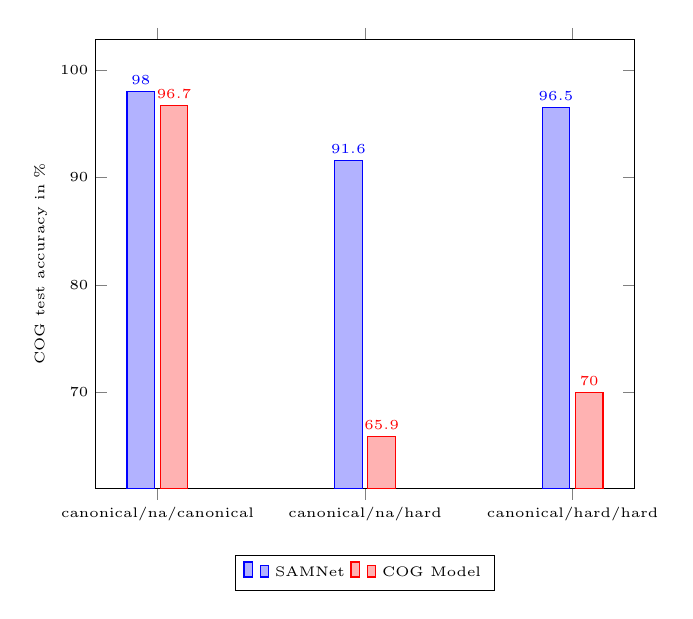
\begin{tikzpicture}
		
				
		\tiny
		
		\begin{axis}[
		ybar,
		enlargelimits=0.15,
		legend style={at={(0.5,-0.15)},
			anchor=north,legend columns=-1},
		ylabel={COG test accuracy in \% },
		symbolic x coords={canonical/na/canonical, canonical/na/hard, canonical/hard/hard},
		xtick=data,
		nodes near coords,
		nodes near coords align={vertical},
		]
		\addplot coordinates {(canonical/na/canonical,98) (canonical/na/hard,91.6) (canonical/hard/hard,96.5)};
		\addplot coordinates {(canonical/na/canonical,96.7) (canonical/na/hard,65.9) (canonical/hard/hard,70)};
		\legend{SAMNet ,COG Model}
		\end{axis}
		\end{tikzpicture}
	}
\end{figure}



